\section{Introduction}
\label{sec:introduction}

Agentic evolution reframes LLM-based problem solving as a process of constructing and revising solutions~\citep{liu2025advances, gao2025evolvesurvey}. 
Instead of treating the model only as a generator of candidate answers, these methods use LLMs, agentic workflows, or coding agents to drive iterative improvement: produce candidate artifacts, interpret feedback from evaluation, and influence what the system explores next~\citep{qu2026coral}. 
This paradigm has been applied to program synthesis~\citep{jimenez2023swe}, scientific discovery~\citep{lu2024ai, yuksekgonul2026learning}, systems optimization~\citep{tbench_2025, deng2025interactcomp}, and agent self-improvement~\citep{zhang2026hyperagents, wang2025huxley, ruan2026aorchestra}. 
In this paper, we use \textbf{agentic evolution} to broadly refer to evolution processes whose search behavior is driven by either structured agentic procedures or general-purpose agents.

Existing agentic evolution methods typically instantiate this paradigm in two ways.
In \textbf{procedure-based evolution}, a predefined outer loop controls parent selection, candidate generation, evaluation, and population update~\citep{novikov2025alphaevolve, ye2026evaluation, zhang2024aflow}.
This makes evolution modular and reproducible, but also ties long-horizon search to fixed selection rules, feedback summaries, and update heuristics.
In \textbf{agent-based evolution}, a general-purpose agent manages the search process by observing feedback, inspecting traces, editing candidates, writing tools, and deciding what to try next~\citep{karpathy2026autoresearch, qu2026coral}.
This gives evolution greater flexibility, but the agent can drift as candidates, logs, hypotheses, and intermediate files accumulate.
In both cases, long-horizon evolution remains prone to local optima: procedures may repeatedly exploit the same hand-designed search pattern, while agents may overcommit to misleading evidence or stale assumptions in a growing context.


Recent work has tried to address these limitations by either broadening exploration with collaborative agents~\citep{qu2026coral} or making the evolution mechanism self-modifying~\citep{zhang2026hyperagents}.
These directions show that stronger search context and editable improvement mechanisms are useful, but they do not by themselves provide a stable interface for long-horizon evolution.
The core challenge is that evolution accumulates candidates, feedback, traces, failures, and intermediate decisions over time, yet lacks a unified way to organize this evidence and revise the mechanism that drives future evolution.


\begin{figure}[!t]
\centering
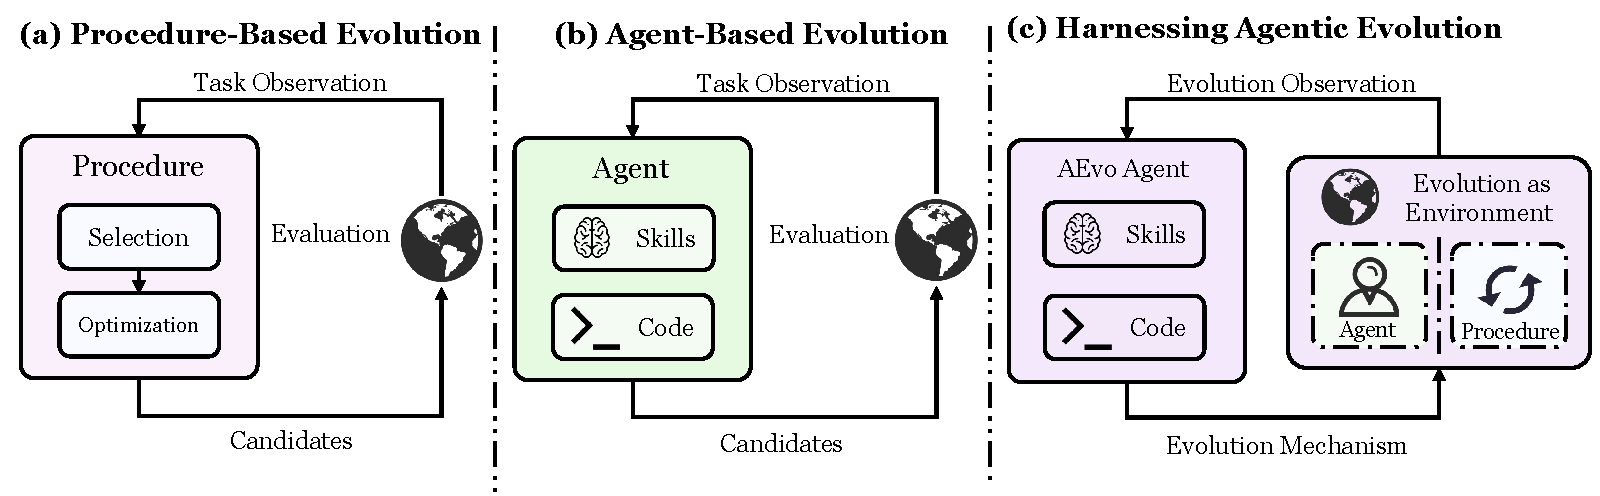
\includegraphics[width=\linewidth]{images/Figure-1.pdf}
\caption{
\textbf{Harnessing agentic evolution as an interactive environment.}
(a) Procedure-based evolution runs a fixed loop for selection, optimization, evaluation, and update.
(b) Agent-based evolution lets a general-purpose agent manage search through feedback, tools, skills, and code actions.
(c) \method treats the evolution process as an interactive environment.
The accumulated evolution context becomes process-level state, while a meta-agent edits the underlying procedure or agent operating context that controls future evolution.
}
\label{fig:teaser}
\end{figure}

We address this challenge by formulating \textbf{agentic evolution as an interactive environment}.
As illustrated in Figure~\ref{fig:teaser}, this view shifts evolution from an unstructured iterative process into an environment that exposes process-level state and supports external intervention.
The state is the accumulated evolution context, including candidates, feedback, traces, failures, costs, and search history.
The transition mechanism is the current evolution mechanism: either an explicit search procedure or the operating context that shapes a general-purpose agent's future decisions.
A meta-agent acts on this environment not by generating the next candidate, but by editing the mechanism that controls how future evolution proceeds.
This makes the same environment view applicable to both hand-designed procedures and general-purpose evolution agents.

Realizing this view requires a harnessed design.
The evolution environment is large, noisy, and constantly changing.
Without a stable interface, a meta-agent may lose track of reliable evidence, revisit old attempts or make edits whose effects are hard to verify.
At the same time, evaluation and candidate records must remain protected from the agents that modify the evolution process.
These challenges motivate a harness that makes evolution observable, editable, and externally governed.

We therefore introduce \method, a harnessed framework for meta-editing agentic evolution.
\method standardizes the evolution workspace, protects the evaluator, records every evaluated candidate into a searchable history, and exposes process-level information to the meta-agent.
It then runs evolution through a two-phase loop. 
In the meta-editing phase, the meta-agent edits the current mechanism and specifies how the next segment should run.
In the evolution segment, the updated mechanism runs under this plan and produces multiple candidates before the next meta-agent intervention.
The same loop can revise both procedure- and agent-based evolution, reducing the risk of local optima.


Our contributions are threefold.
(1) \textbf{Environment Formulation:} We formulate agentic evolution as an interactive environment, where accumulated evolution context becomes process-level state and meta-actions edit the mechanism that drives future evolution.
(2) \textbf{Harnessed Meta-Editing:} We introduce \method, a harnessed framework for meta-editing agentic evolution that protects evaluation, records evaluated candidates, and supports coarse-grained intervention through meta-editing phases and evolution segments.
(3) \textbf{Cross-Form Instantiation and Evaluation:} We instantiate the same framework on both procedure-based and agent-based evolution, showing that \method can revise either explicit procedure components or agent operating contexts.
On standard agentic and reasoning benchmarks, \method outperforms five evolution baselines and achieves a 26\% relative improvement over the strongest baseline.
On three open-ended optimization tasks, \method outperforms four evolution baselines and achieves state-of-the-art performance under the same iteration budget.